\documentclass{article}
\usepackage{tikz, pgfplots}
\usetikzlibrary{arrows}
\begin{document}
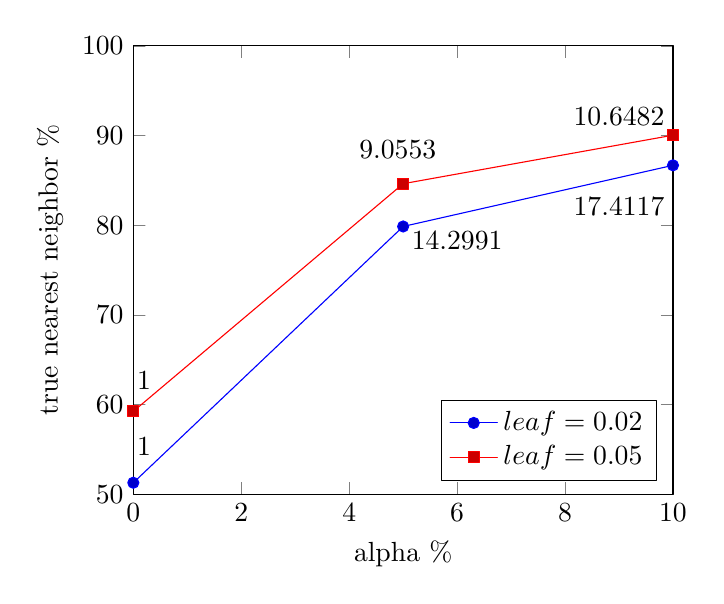
\begin{tikzpicture}[line cap=round,line join=round,>=triangle 45,x=1.0cm,y=1.0cm]
\begin{axis}[
xlabel=alpha \%,
xmin=0,
xmax=10,
ylabel=true nearest neighbor \%,
ymin=50,
ymax=100,
legend pos=south east]
\addplot coordinates{
(0,		51.27)
(5,	    79.85)
(10,    86.67)
};
\addlegendentry{\(leaf=0.02\)};
\addplot coordinates{
(0,		59.23)
(5,	    84.62)
(10,	90.03)
};
\addlegendentry{\(leaf=0.05\)};
\node[above]at(axis cs: 0.2, 53.27){\(1\)};
\node[below]at(axis cs: 6,   80.35){\(14.2991\)};
\node[below]at(axis cs: 9,   84.2){\(17.4117\)};
\node[above]at(axis cs: 0.2, 60.53){\(1\)};
\node[above]at(axis cs: 4.9, 86.32){\(9.0553\)};
\node[above]at(axis cs: 9,   90.03){\(10.6482\)};
\end{axis}
\end{tikzpicture}
\end{document}
